\section{Signal Extraction}
\label{sec:signalextraction}
The signature for the decay $\Hgg$ is the presence of a narrow peak on a smoothly falling background in 
the invariant mass spectrum. 
The signal to background ratio can be dramatically increased by focusing on events falling in a window 
around the mass of the Higgs boson, $m_{H}$. Since this mass is not predicted in the Standard Model, 
the search is performed for a range of mass hypotheses effectively sliding the signal window across 
the diphoton invariant mass spectrum, $\mgg$.
As the signal yield for a SM Higgs boson decaying to two photons is small, 
additional event information from the detector and the kinematics of the diphoton system can be used to 
increase the sensitivity of the search. 

This section describes a multivariate analysis (MVA) based approach to extracting the signal, categorizing events within a sliding 
signal window based on a single event discriminator (categorisation BDT). The approach allows for use of data in sidebands
to determine expected event yields within the signal region, making few assumptions about the specific
composition and kinematics of the background. This approach is the second of the two methods (method B) for extracting the signal, used by the CMS $\Hgg$ group.

\subsection{Definition of the Signal Region}

Once the expected resolution of the $\Hgg$ peak is determined, the choice of signal window can be optimized
to reduce the uncertainty on the background while selecting as many signal events as possible.
The size of the signal window is chosen using a simplified analysis in which the number of signal events
from a SM Higgs boson with hypothesised mass $m_{H}$ expected within the range $|\Delta M/M_{H}|=|(\mgg-m_{H})/m_{H}| < w$ 
is compared to the uncertainty on the total number of events (from background and signal) in that range.
The figure of merit, $N_{S}/\sigma = N_{S}/\sqrt{\sigma_{S}^{2} + \sigma_{B}^{2}}$, is calculated as
a function of signal region cut value, $w$, for a range of mass hypotheses as shown in Figure~\ref{fig:sigwindowopt}. 
The error on the number of background events, $\sigma_{B}$, is calculated using the procedure described in 
Section~\ref{sec:backgroundmodel} whereas the error on the signal is purely statistical.
For this analysis, $w=0.02$ was chosen as the optimal signal region cut value.

\begin{figure}
 \begin{center}
  \includegraphics[width=0.9\textwidth]{hgg7TeV/sidebandMvaPlots/fom.pdf}
 \end{center}
  \caption{Figure of merit for selection of the signal region cut value, $w$. Each colour shows the evaluation
  under different Higgs boson mass hypotheses.}
  \label{fig:sigwindowopt}
\end{figure}


\subsection{Event Categorisation BDT}
\label{sec:bdteventdiscriminator}

The inputs to the diphoton BDT contain information from the event kinematics and the quality of the photons 
and vertex location in the form of the photon ID BDT output and event resolution estimators. 
The output of the diphoton BDT combined with the invariant mass of the diphoton system therefore provides 
the necessary information to separate signal from background.

Figure~\ref{fig:bdtplane} 
shows the variation in the signal to background ratio ($S/B$) across different regions in the 
two-dimensional plane defined by the output of the diphoton BDT and $\dmom$.
Events close to the centre of the peak ($\dmom=0$) with a high score in the diphoton BDT are more
likely signal events than those far from the high $S/B$ regions.

\begin{figure}
\begin{center}
  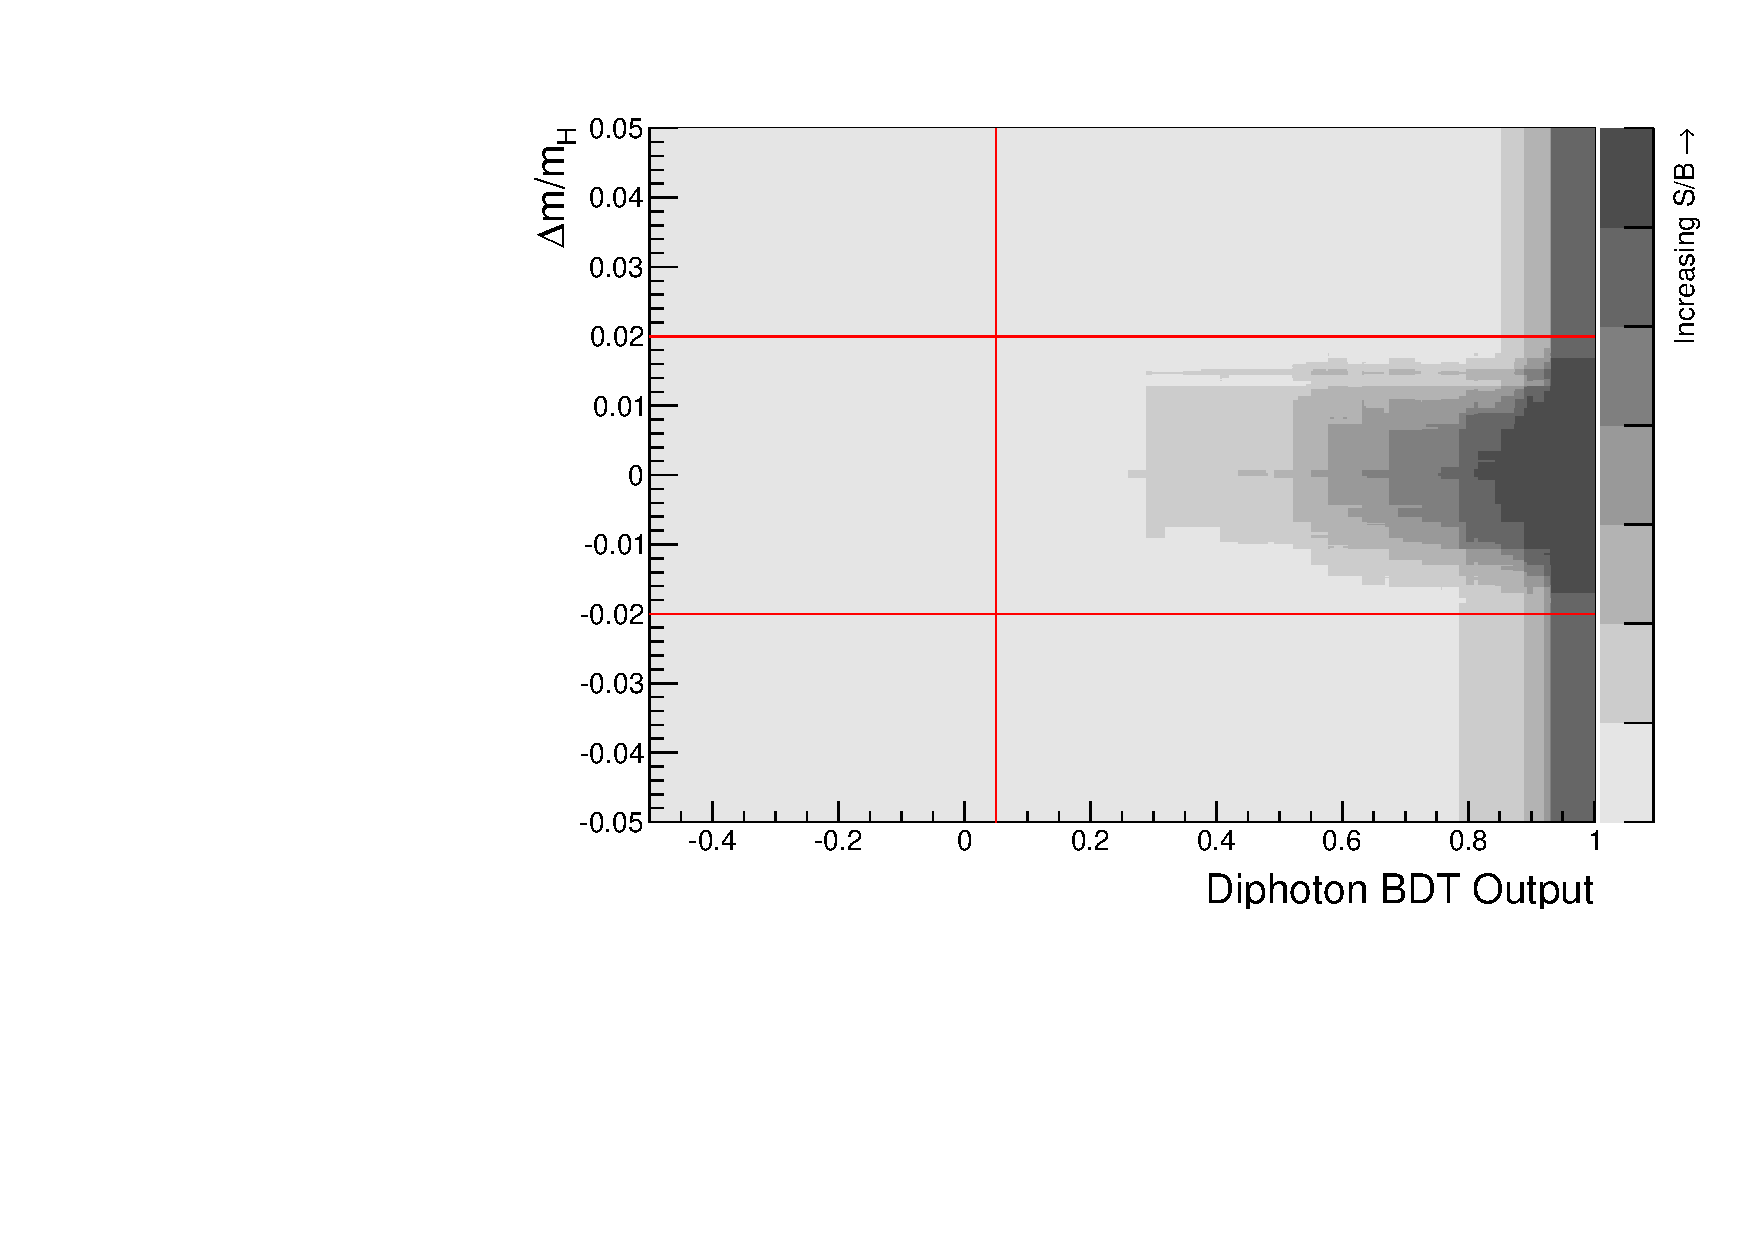
\includegraphics[width=0.8\textwidth]{hgg7TeV/sidebandMvaPlots/bdt2dplot.png}
\end{center}
 \caption{Signal to background ratio as a function of diphoton BDT output and $\dmom$.
 The red lines indicate the cuts applied before the training and for applying the event selection. 
Darker shades indicate a regions with a higher signal to background ratio. The seven shades indicate the 
region contained in each of the seven BDT bins used for the signal extraction at $m_{H}= 123$ GeV.}
 \label{fig:bdtplane}
\end{figure}

The two variables are combined to produce a single event discriminator by training a BDT using the 
diphoton BDT output and $\dmom$ as inputs. 
The BDT is trained with Higgs signal MC with $m_{H}=123$ GeV including all four production processes 
and background MC including prompt-prompt, prompt-fake and fake-fake events.
The performance of several different training methodologies was compared to find which gave the 
optimum separation of signal and background.
Two different choices of boosting were studied, adaptive and gradient boosting, both of which 
weight decision trees to optimize the performance in terms of signal-background separation~\citep{tmva}. 
In addition, these were compared to a simple likelihood 
which does not account for correlations between the 
diphoton BDT and $\dmom$ as shown in Figure~\ref{fig:mvacomparisons}.
The gradient boosting method was found to give the best performance although the variation between 
methodologies is small.
 
\begin{figure}
\begin{center}
  \includegraphics[width=0.8\textwidth]{hgg7TeV/sidebandMvaPlots/roc}
\end{center}
 \caption{Signal efficiency vs background rejection curves for three different MVA techniques used to train
 the signal-background event discriminator. The curves give the (in)efficiencies for signal (background) 
 after applying sequentially tighter cuts on the discriminator output.}
 \label{fig:mvacomparisons}
\end{figure}

With finite statistics, a BDT can be over-trained by allowing the training to emphasise statistical fluctuations which are not physical and will not necessarily be
representative of the data. To test for this, the MC samples are split into two equal samples, the first of which is used to train the BDT. The distribution 
of the output values of the BDT from the second set is compared to that of the training sample as shown in Figure~\ref{fig:bdttraining}. The comparison
is shown using both an arbitrary binning scheme and the final set of bins derived in 
Section~\ref{sec:binningofthebdtoutputdistribution}.
A $\chi^{2}$ test was performed on the distributions with the final bins giving p-values of 0.06
for the background and 0.95 for the signal indicating that over-training has not occurred.

\begin{figure}
\begin{center}
  \includegraphics[width=0.48\textwidth]{hgg7TeV/sidebandMvaPlots/testvstrain_nolegend}
  \includegraphics[width=0.48\textwidth]{hgg7TeV/sidebandMvaPlots/testvstrain-finalbins-neat}
\end{center}
 \caption{Signal and background BDT output distribution with the training sample (points)
and testing sample (solid area) superimposed. The comparison is shown 
using an arbitrary uniform binning (left) and the bins used for extracting the signal (right).}
 \label{fig:bdttraining}
\end{figure}

In this analysis, the background is estimated entirely from data. This means that disagreement between
data and background MC will affect the performance of the BDT rather than the validity of the final results. 
The agreement between the data and MC is shown in Figure~\ref{fig:datamcagreement_sidebandBDT} for the mass 
hypothesis, $m_{H}=125$ GeV. The level of agreement is sufficient so as not to require in-depth study of the
BDT output distributions of the background MC.

\begin{figure}
 \begin{center}
  \includegraphics[width=.8\textwidth]{hgg7TeV/sidebandMvaPlots/data-mc-sbsum-mh125}
 \end{center}
 \caption{Comparison of the distributions of BDT output at $m_{H}=125$ GeV for data and background MC. 
 The distributions are arbitrarily binned for the purposes of comparison only.}
 \label{fig:datamcagreement_sidebandBDT}
\end{figure}

\subsection{Binning of the BDT Output Distribution}
\label{sec:binningofthebdtoutputdistribution}

The BDT provides a single variable with which to classify events based on their signal to background 
ratio, $S/B$, which will have a discrete number of response values based on the number of
trees used. The boosting procedure provides a pseudo-continuous distribution which is used
to model the signal and background. However, the resulting distribution will still be only
pseudo-continuous. In addition, the BDT response does not directly correspond to a physical
distribution and it is therefore difficult to motivate any parameterisation of either the signal
or background distributions. To overcome these issues, a binning procedure is defined to 
construct templates which are used as models for the signal and background expectation as a
function of BDT response range (BDT bin). This procedure is designed firstly to ensure that no
bin has zero background expectation and secondly that as few bins as possible
are used without reducing the sensitivity of the BDT. 
These requirements are desirable such that 
the expected background yield in each bin can be derived using data outside of the signal region
as described in Section~\ref{sec:backgroundmodel}.

A scan is performed in which the definitions of the bin boundaries are varied in order to
find the maximum expected significance in the presence of a SM Higgs signal. For $N$ bins 
($N-1$ boundaries) with background and signal expectation yields $b_{i}$ and $s_{i}$ respectively,
the expected significance, $\sigma_{exp}$, is given by

\begin{equation}
 \sigma_{exp} = \left( 2 \sum_{i=1}^{N} (s_{i}+b_{i})\ln\left(\frac{\displaystyle s_{i}}{\displaystyle b_{i}} +1\right) - s_{i} \right)^{1/2},
\label{eqn:expectedsig_bins}
\end{equation}
using the log-likelihood ratio for Poisson likelihoods.
The binning procedure is defined as follows:

\begin{enumerate}

\item The distribution of background MC is binned very finely to provide an almost discrete
dataset (5000 equally spaced bins are used). The background is re-binned such that there are 20
expected events per bin at a luminosity of \clumi. 
\item Smoothed versions of the signal (at each 5 GeV step mass) and background MC templates are produced 
in order to obtain a stable model of $S/B$ as a function of BDT bin.
The smoothing procedure is done via binning a fit (of a 9th order polynomial) to the signal
distribution.
\item $N$ bin edges (boundaries), $b_{i}$, are defined on the remaining bins such that $N+1$ bins 
are formed with $b_{1} < b_{2} < \ldots < b_{N}$. The first bin is defined as $[-1,b_{1})$ and the last
is defined as $[b_{N},1]$. The $N$ dimensional scan is performed varying these
bin edges to find the maximum expected significance in the presence of a SM Higgs signal. 
\item An extra boundary is added, the scan is repeated and the maximum expected
significance is found for $N+1$ boundaries. If the maximum expected significance  
is increased by more than 0.1\% compared to that of step 3, the new boundary is kept and step 4 
is repeated, if not, the procedure terminates.
\end{enumerate}

The scan in step 3 is split into two parts, first using a large step size to find the 
region where the maximum lies followed by a fine scan in small steps within that region. 
The ratio of small to large step size is chosen to be that
which minimizes the total number of iterations in the scan to reduce the time taken for the procedure.
An example of the binning procedure is shown in Figure~\ref{fig:binningscheme}. 
The red histogram is the $S/B$ distribution after step 1, the 
blue after step 2 and the black vertical lines show the final set of 7 bins chosen for this analysis.
Dijet tagged events are treated in the same way as the rest of the events in the analysis 
by introducing an eighth bin containing events from any BDT output bin inside the range $\dmom < w$ 
which pass the dijet tag.

\begin{figure}
 \begin{center}
  \includegraphics[width=0.8\textwidth]{hgg7TeV/sidebandMvaPlots/binningscheme.pdf}
 \end{center}
 \caption{Signal to background ratio as a function of BDT output bin.
 The red and blue histograms show the distribution after applying step 1 of the binning procedure before
and after smoothing respectively. The black vertical lines indicate the boundaries of the final
binning choice from the full procedure.}
 \label{fig:binningscheme}
\end{figure}


\subsection{Background Model}
\label{sec:backgroundmodel}

The SM background is expected to have a smoothly varying invariant mass spectrum.
However, detector effects such as selection, trigger efficiencies and energy resolution 
shape this distribution in ways which are imperfectly modelled in MC simulation.
Moreover, the background contains fakes whose contribution varies as a function of $\mgg$.
This means the exact composition of the background is needed to model the shape with MC.
In order to remove the impact of systematic uncertainties associated with this, an entirely data-driven
approach for modelling the background is used.

For a given mass hypothesis, the shape and normalization of the background model are obtained separately. 
The shape, meaning the fraction of events in each BDT output bin, is extracted
from the BDT output distributions in mass-sidebands, while the overall normalization is obtained
from a parametric fit to the mass distribution for all selected events excluding the signal region.

Figure~\ref{fig:fullmassspec} shows the invariant mass distribution after event selection in the range 
$100 < \mgg < 180$ GeV for the full 2011 dataset. The red band indicates the signal region for
$\mh=124$ GeV, while the six blue bands indicate the corresponding sidebands used to determine the shape 
of the background model. 
The blue line indicates the fit of a sum of two power laws which is used to determine the normalisation of the
background in the signal region.

\begin{figure}
 \begin{center}
  \includegraphics[width=.8\textwidth]{hgg7TeV/sidebandMvaPlots/fits/massfit.pdf}
 \end{center}
 \caption{Invariant mass distribution of the full 2011 dataset after selection over the mass range used in
the analysis (100 to 180 GeV). The $\pm 2\%$ signal region for $\mh=124$ GeV is indicated in red, while the six
corresponding sidebands are indicated as blue bands. The blue line is the double power law fit to the data for 
the background normalisation for this mass hypothesis.}
 \label{fig:fullmassspec}
\end{figure}

\subsubsection{Obtaining the Normalisation of the Background}
\label{sec:backgroundnormalisation}

The normalisation of the background model is estimated using an un-binned maximum likelihood fit of
a parametric function to the diphoton invariant mass distribution in the range $100 < \mgg < 180$ GeV. 
The normalisation 
of the background model is given by the integral of the function over the $\pm2\%$ signal region
for each mass hypothesis. The  signal region is excluded from the fit to avoid potential bias in the 
presence of a signal.

The particular parameterization used was chosen following a study of different parametric forms which also provide a good
fit to the data. Since the actual functional form is unknown, the choice of parameterization is taken to be
that which minimises the total uncertainty when comparing to the other functional forms.
Twelve different functional forms were considered, which can be grouped into four general classes:
exponentials, power laws, real Laurent polynomials and standard polynomials. Within each of these
classes, three functions were used. For the exponentials and power law cases, these were sums
of one, two or three exponential or power law ($\mgg^{-r}$) terms, while only first, third and fifth order
standard polynomials were used. 
For the Laurent polynomials, the functions were sums of two, four or six terms, specifically
\begin{eqnarray*}
\mgg^{-4}+a\mgg^{-5},\\
\mgg^{-4}+a\mgg^{-5}+b\mgg^{-3}+c\mgg^{-6},\\
\mgg^{-4}+a\mgg^{-5}+b\mgg^{-3}+c\mgg^{-6}+d\mgg^{-2}+f\mgg^{-7}.
\end{eqnarray*}
For each class therefore, the three functions have one, three or five parameters for the shape.

To assess the bias introduced through choosing one particular parameterisation, pseudo-experiments are
generated from each functional form and the invariant mass of those experiments are
fit with the other functional forms. The parameters for generation of the pseudo-experiments are 
fixed by fitting each functional form to the data in the full mass range.
In each pseudo-experiment, the integral of a particular fitting function, A, over the signal region is 
compared to that from a generating function, B. The distribution of the difference between the two values
across all of the pseudo-experiments is used to determine the bias introduced from choosing function A when B was the true function. 
The distributions are then weighted according to the probability of the initial fit to the data 
and combined so that the total uncertainty from choosing a particular function is computed as the RMS from 
zero of the weighted summed distributions for all generating functions. Since one of the generating functions
can also be the fitting function, the error includes both the statistical uncertainty from the limited data sample
and the systematic uncertainty due to an incorrect choice of parameterisation.
This study is repeated at 5 GeV intervals in $m_{H}$ as the overall uncertainty varies as a function of 
mass hypothesis. Figure~\ref{fig:totalerrorallfunc} shows the total error determined for each of the twelve functions 
at each value of $m_{H}$ tested. The sum of two power laws was found to give a low total uncertainty while also demonstrating 
good fit stability in the pseudo-experiments. The total error on the background normalisation
is included as a single systematic uncertainty for the purpose of signal extraction
(Section~\ref{sec:statisticalinterpretations}).

\begin{figure}
 \begin{center}
  \includegraphics[width=.8\textwidth]{hgg7TeV/sidebandMvaPlots/fits/totalErrors}
 \end{center}
 \caption{Total error on the background normalisation as a function of $m_{H}$ from different choices of the 
background shape parameterisation of $\mgg$. The total error for the one-parameter exponential and polynomial functions are off the scale of this plot.}
 \label{fig:totalerrorallfunc}
\end{figure}


\subsubsection{Obtaining the Shape of the Background}
\label{sec:backgroundshape}

As the signal yield expected from a SM Higgs boson is small compared to the background, 
the sensitivity of the search is strongly dependent on how well the relative contribution
from the background in each bin is understood.
Both inputs to the BDT are designed to be insensitive to the invariant mass of the diphoton system,
therefore the BDT output distribution should be the same for any region of the $\mgg$ spectrum.
Since the background composition remains relatively constant across the range 100 to 180 GeV, 
data in sidebands of $\mgg$, away from the signal, can be defined to determine the BDT  
distribution of the background inside the signal region. For a particular $\mh$, a contiguous
set of lower/upper sidebands are defined to be the ranges $|\dmomsb| < w$ 
centered on $\mhsb$ as given in Equation~\ref{eqn:sbdefsu} where $w=0.02$.
\begin{eqnarray}
	\mhsb = \mh \left( \frac {\displaystyle 1+w }{1-w} \right)^{i} 
\label{eqn:sbdefsu}
\end{eqnarray}
The two sidebands adjacent to the signal window 
(corresponding to $i=\pm1$ in Equation~\ref{eqn:sbdefsu}) are not used in order
to avoid signal contamination. Dijet tagged events are treated in the same way as the rest of the events by introducing an eighth bin
containing dijet tagged events inside the range $\dmom < w$.
The distributions for the two input variables, diphoton BDT output and $\dmom$, 
for each of the six sidebands corresponding to $\mh=125$ are
shown in Figure~\ref{fig:datasidebandsinput}. Each distribution is normalised to unit area. The 
resulting BDT output distributions are shown in Figure~\ref{fig:datasidebandsoutput}. 
The distributions from each sideband are not distinguishable within the statistical 
uncertainties.

\begin{figure}
 \begin{center}
  \includegraphics[width=0.48\textwidth]{hgg7TeV/sidebandMvaPlots/datasidebands_diphobdt}
  \includegraphics[width=0.48\textwidth]{hgg7TeV/sidebandMvaPlots/datasidebands_dmom}\\
 \end{center}
 \caption{Distribution in data from the six sidebands corresponding to $\mh=125$ GeV of the two BDT 
 input variables, diphoton BDT (left) and $\dmom$ (right).}
 \label{fig:datasidebandsinput}
\end{figure}
\begin{figure}
 \begin{center}
  \includegraphics[width=.8\textwidth]{hgg7TeV/sidebandMvaPlots/datasidebands_finalbdt}
 \end{center}
 \caption{Distribution in data from the six sidebands corresponding to $\mh=125$ GeV of the BDT output
 binned in the 7 BDT output bins used for signal extraction.}
 \label{fig:datasidebandsoutput}
\end{figure}

The residual variation in BDT output is due to the small variation in background composition with mass.
This is mostly due to the photon ID BDT distribution being sensitive to the fake component which 
varies with mass. In order to account for this variation, the background model is constructed using 
a simultaneous linear fit to the BDT output shape in the data sidebands.
The expected fraction of events in each bin, $f_{j}$, for a given mass hypothesis, $\mhsb$, is given
by Equation~\ref{eqn:sbfitdef}, where 
$j\epsilon\{1,8\}$ and $i\epsilon\{\cdots,-4,-3,-2,2,3,4\cdots\}$. 
\begin{equation}
f_{j} = p_{0,j} + p_{1,j}(\mhsb - \mh)
\label{eqn:sbfitdef}
\end{equation}
Since the normalisation for the background model is determined independently, 
the sum over all bins is constrained to be one. 
The expectation value for the background in each bin, $j$, is then determined as $Nf_{j}$ where $N$ is the
normalisation estimated in section~\ref{sec:backgroundnormalisation}.
This constraint is imposed for all $\mhsb$ by fixing
\begin{eqnarray} 
 p_{0,1} = 1-\sum_{i=2}^{8} p_{0,j} &&  p_{1,1} = - \sum_{j=2}^{8}p_{1,j}
\end{eqnarray}
The coefficients $p_{0,j},p_{1,j}$ of Equation~\ref{eqn:sbfitdef} are determined by performing a binned
maximum likelihood fit to the observed fractions in the data assuming the contents of each bin in each 
sideband are Poisson distributed. The results of the fit for $\mh=124$ GeV are shown in 
Figure~\ref{fig:examplesbfits} and the resulting covariance matrix obtained is shown in 
Figure~\ref{fig:covariance}. 
The fit was performed using \texttt{TMinuit} under \texttt{ROOT 5.2.0}~\citep{minuit}. 

\begin{figure}
 \begin{center}
  \includegraphics[width=0.46\textwidth]{hgg7TeV/sidebandMvaPlots/fits/m124_bg_bdt_bin_1}
  \includegraphics[width=0.46\textwidth]{hgg7TeV/sidebandMvaPlots/fits/m124_bg_bdt_bin_2}\\
  \includegraphics[width=0.46\textwidth]{hgg7TeV/sidebandMvaPlots/fits/m124_bg_bdt_bin_3}
  \includegraphics[width=0.46\textwidth]{hgg7TeV/sidebandMvaPlots/fits/m124_bg_bdt_bin_4}\\
  \includegraphics[width=0.46\textwidth]{hgg7TeV/sidebandMvaPlots/fits/m124_bg_bdt_bin_5}
  \includegraphics[width=0.46\textwidth]{hgg7TeV/sidebandMvaPlots/fits/m124_bg_bdt_bin_6}\\
  \includegraphics[width=0.46\textwidth]{hgg7TeV/sidebandMvaPlots/fits/m124_bg_bdt_bin_7}
  \includegraphics[width=0.46\textwidth]{hgg7TeV/sidebandMvaPlots/fits/m124_bg_bdt_bin_8}
 \end{center}
 \caption{Simultaneous fits to the six sidebands in data to determine the background shape for 
$\mh=124$ GeV. There are eight panels showing the result in each of the seven BDT bins plus one for 
the dijet tagged bin. The six black points in each panel are the fractional populations 
of the data in each sideband. The blue line represents the linear fit used to determine the fraction
of background in each bin.}
 \label{fig:examplesbfits}
\end{figure}

\begin{figure}
 \begin{center}
  \includegraphics[width=.8\textwidth]{hgg7TeV/sidebandMvaPlots/fits/covariance_m124}
 \end{center}
 \caption{Covariance matrix from the sideband fit to determine the background shape at
 $\mh=124$ GeV. The covariance matrix includes the additional 20\% systematic attributed to possible second
 order variations in the BDT output background distribution with mass.}
 \label{fig:covariance}
\end{figure}

There are seven degrees of freedom (eight bins minus one constraint) which are correlated in the simultaneous fit.
In order to account for the statistical uncertainty on this fit, a set of seven uncorrelated variables
are determined from the covariance matrix using eigenvector decomposition~\citep{pca}. These variables 
are treated as seven independent sources of systematic uncertainty on the background shape
for the purpose of signal extraction (Section~\ref{sec:statisticalinterpretations}). 
Figure~\ref{fig:relativefiterrorvsnsidebands} shows the total relative fit error for each bin, 
at $\mh=130$ GeV, as the number of 
sidebands, is varied.
Increasing the number of sidebands beyond six, three on each side of the signal region,
provides negligible reduction in the statistical uncertainty.
In order to avoid contamination from $\Zee$ at the lower mass hypotheses
any lower sideband whose lower boundary is less than 100 GeV is removed and an additional higher
sideband is introduced. Consequently mass hypotheses in the range $111 \le \mh < 115.5$ have
two lower and four upper sidebands and mass hypotheses in the range $110 \le \mh < 111$ have
one lower and five upper sidebands.

\begin{figure}
 \begin{center}
  \includegraphics[width=.8\textwidth]{hgg7TeV/sidebandMvaPlots/fits/fracErrorvsNsidebands.pdf}
 \end{center}
 \caption{Relative total fit uncertainty on the background model in each bin at $\mh=130$ GeV as a function of the 
 number of sidebands used in the fit to determine the shape of the background.}
 \label{fig:relativefiterrorvsnsidebands}
\end{figure}

At most linear variations with mass are considered for the background BDT output distribution.
This corresponds to evaluating the first term in a Taylor series for the true shape of the distribution
about $\mh$. Higher terms can be introduced but the statistical precision of the fit will be reduced in 
doing so. To check for potential significant deviations in the data from linearity, pseudo-experiments
were generated in which the expected fractions, $f_{i}$ are assumed to follow,
\begin{equation}
f_{j} = p_{0,j} + p_{1,j}(\mhsb - \mh) + \frac{\displaystyle 1}{\displaystyle 2} p_{2,j}(\mhsb-\mh)^{2}.
\label{eqn:sbfitdefho}
\end{equation}
The parameter values, $p_{0,j},p_{1,j}$ and $p_{2,j}$ and their uncertainties were determined 
by fitting over a larger
number of sidebands for a particular mass hypothesis. This is done by extending the range of $j$ to allow
any sideband which is contained inside the range $100 < \mgg < 180$ GeV. For most mass hypotheses, this 
corresponds to fifteen sidebands in total. For each pseudo-experiment, the parameters were varied 
within their uncertainties (accounting for correlations) thereby systematically altering the expectation
value for the number of events in each bin before generating a Poisson toy for the observed number of 
events per bin in each sideband. The usual linear fit is then performed and the fraction of events in each
bin for the signal region is extracted and compared to the true generating fraction. The difference between these
two values can be used to determine the total error under the assumption
that a second term in the Taylor expansion is present in the data. This error is taken as the root mean square 
(RMS) around zero
of the difference between the true and fitted values for $f_{i}$ in 10,000 pseudo-experiments. When compared
to the error from the linear fits, it was found that the total uncertainty was covered by inflating
the errors systematically by 20\%. The value of 20\% is a conservative choice being the largest value 
found when repeating the study over a range of mass hypotheses. 

\subsection{Signal Model}
\label{sec:signalmodel}

The signal model for the Higgs boson decay to two photons at a given mass is constructed by 
binning the BDT response from MC simulation of the four production processes, $ggH$, $qqH$, $VH$ and $ttH$.
The simulation is corrected using auxiliary
measurements from $\Zee$ events in data to account for imperfect modeling of the detector.
These corrections are applied to the Monte Carlo event by event and can be categorized into
photon and diphoton level corrections.

\subsubsection{Photon Level Corrections}
The energy resolution of the calorimeter is measured in data using $\Zee$ events in
categories defined by the position and $\rnine$ of the supercluster. 
Photons in the central region of the detector
with $\rnine > 0.94$ are further divided into those whose supercluster seed lies close to a module 
boundary and those whose does not. 
The additional energy smearing required for the Monte Carlo in each category is determined
by smearing $\Zee$ MC until the $e^{+} e^{−}$ invariant mass distribution matches that
of the data. 
This additional resolution is included in the Higgs MC by scaling the energy of each photon by 
$G(1,\sigma_{cat})$ where $G$ is a Gaussian distributed random variable centered
at 1, and $\sigma_{cat}$ is the additional resolution required to match the data in a particular category.
The exact definitions of the photon-level categories and the additional resolution measured in each category
are given in Table~\ref{tab:eres2011}.
 
The efficiency for a photon to pass the pre-selection is measured in $\Zee$ data in four categories.
These are defined by whether or not the supercluster is in the ECAL barrel or either endcap and the value 
of $\rnine$ being greater or less than 0.94. 
The ratio of the efficiency measured in data to that measured in MC provides a scale factor which is
applied to the signal MC. Each signal event is reweighted by the product of the scale factors
for each photon in the selected diphoton pair. In addition to these corrections, the value of $\sigma_{E}$ and the photon ID BDT for each photon is 
shifted in each signal event to account for imperfections in detector simulations as described in 
Section~\ref{sec:diphotonbdt}.

\subsubsection{Diphoton Level Corrections}
The efficiency to select the correct vertex in the event is measured using $\Zmumu$ events as a
function of the boson $p_{T}$ as described in Section~\ref{sec:vertexselection}. 
Signal MC events are categorized by whether or not the 
selected vertex is within 10mm of the generated vertex. Each event is then re-weighted by
the ratio of the probability that the event lies in a particular category
as measured in $\Zmumu$ data ($\epsilon_{data}$) to that measured in $\Zmumu$ MC ($\epsilon_{MC}$). Figure~\ref{fig:vtxprobreweight} 
shows the weight, $\epsilon_{data}/\epsilon_{MC}$, applied to events in the signal MC in which the correct vertex is selected
as a function of the Higgs boson candidate $\pt$ ($\pth$). Similarly, events in which this is not
the case are reweighted by the ratio  $(1-\epsilon_{data})/(1-\epsilon_{MC})$. 
The L1/HLT efficiency is measured in four diphoton categories depending on the maximum
supercluster $\eta$ and minimum $\rnine$ value of the two photons using $\Zee$ data. 
As the simulation does not include the trigger, the efficiency is applied 
directly as a weight to each MC event.

\begin{figure}
\includegraphics[width=0.8\textwidth]{hgg7TeV/generalPlots/vtxReweight.pdf}
\caption{Re-weighting applied to signal MC in which the $z$ position of the selected vertex 
is within 10mm of the true vertex as a function of $\pth$. The weights are derived from $\Zmumu$ events
 in data and MC.}
\label{fig:vtxprobreweight}
\end{figure}

\subsubsection{Systematic Uncertainties}

For each correction applied to the MC, the accuracy to which that correction
is measured provides an estimate of the uncertainty present in the signal model. 
In the case of the energy scale measurement, no correction is applied to the MC although the 
uncertainty in that measurement is treated as a systematic on the per-photon energy in signal MC events.
The systematic uncertainties that affect the shape of the signal are treated as correlated  
migrations across the BDT output bins. The effect of each systematic in each
bin is derived by shifting the relevant quantity in the signal MC and recalculating the BDT output for each event.
The difference between the signal yield in each bin after applying the shift quantifies the variation due to that uncertainty.
In practise, these quantities are derived by applying shifts to the MC corresponding to $3\sigma$ variations 
of each uncertainty and interpolating the difference from the nominal values back to the $1\sigma$ level.
This is done so that the evaluation of the variation in each bin is more robust for systematics which 
have a small effect on the BDT output and in signal processes with fewer available MC events.
Figure~\ref{fig:signalmodel_escaleres} shows the effect of the energy scale and resolution uncertainties
on the BDT output of signal from gluon-gluon fusion production.

\begin{figure}
\begin{center}
  \includegraphics[width=0.48\textwidth]{hgg7TeV/sidebandMvaPlots/signalModel/systematic_interpolation_test_E_scale.pdf}
  \includegraphics[width=0.48\textwidth]{hgg7TeV/sidebandMvaPlots/signalModel/systematic_interpolation_test_E_res.pdf}
  \includegraphics[width=0.48\textwidth]{hgg7TeV/sidebandMvaPlots/signalModel/systematic_interpolation_test_curves_E_scale.pdf}
  \includegraphics[width=0.48\textwidth]{hgg7TeV/sidebandMvaPlots/signalModel/systematic_interpolation_test_curves_E_res.pdf}
\end{center}
 \caption{Top: Energy scale (left) and resolution (right) uncertainties in the $ggH$ signal model. 
The effect of $\pm3\sigma$ variations 
derived in MC are shown with red dashed lines while the interpolated $\pm3\sigma$ are shown with blue.
Bottom: Variation in bin content at different quantiles (number of standard deviations from the nominal) for the
three highest $S/B$ BDT bins. 
The blue and red markers indicate the yields extracted directly from MC while the black line indicates the 
quadratic interpolation function used to derive the $\pm1\sigma$ variations for the signal model.}
 \label{fig:signalmodel_escaleres}
\end{figure}

Imperfections in the simulation of the shower shape variables can cause discrepancies in the photon 
ID and $\sigma_{E}$ distributions obtained from the respective BDTs between data and MC. To account for this, 
systematic uncertainties are included corresponding to shifting or scaling the output of the photon ID BDT 
and regression BDT respectively and recalculating the BDT output for each event in signal MC. The size 
of the uncertainty is chosen to be that which covers the maximal difference in the ratio of each 
distribution for high $\pt$ photons. This is then validated using $\Zee$ events in which the 
electrons are reconstructed as photons.
The overall efficiency$\times$acceptance after applying 
these scale factors is shown as a function of $\mh$ in Figure~\ref{fig:effacc}. 
\begin{figure}
\includegraphics[width=0.8\textwidth]{hgg7TeV/generalPlots/effAcc_vs_mass.pdf}
\caption{Efficiency$\times$acceptance for a SM Higgs boson as a function of its mass ($\mh$) after
applying all of the corrections to the MC. The blue bands indicate the error from each source of 
systematic uncertainty on the signal model summed in quadrature.}
\label{fig:effacc}
\end{figure}
Due to the large variations observed when using different underlying event parton showering (UEPS) models
for the two dominant production processes, systematics of 70\% and 10\% are included as the uncertainty
in the fraction of gluon-gluon fusion and vector boson fusion events respectively which
are expected to pass the dijet tag~\citep{HIG-11-033}.
In addition to the shape systematics, theoretical errors on the SM Higgs boson cross-section are 
included due to uncertainties on the QCD scale and pdf variations of the various
production modes~\citep{lhcxswg}. A 2.2\% luminosity error is also included as an uncertainty
on the overall signal yield.
A complete list of the systematics included in the signal model is given in Table~\ref{tab:sigsystematics}.

\begin{table}[htbp]
\begin{tabular}{| l r|c|c|}
\hline
\multicolumn{2}{| l |}{{\textbf{Source of systematic uncertainty}}} & \multicolumn{2}{ c |}{{\textbf{Uncertainty}}}\\  
\hline
\hline
%%%%%% per photon ----------------
\multicolumn{2}{| l |}{{\textbf{Per photon}}} & Barrel & Endcap \\  
\hline
\multicolumn{2}{| l |}{Photon identification efficiency} & 1.0\% & 2.6\%\\
\hline
%\hline
Energy resolution  & $\rnine > 0.94$ (low $\eta$, high
$\eta$) & \small{0.22\%, 0.61\%} & \small{0.91\%, 0.34\%} \\
($\Delta\sigma/E_{MC}$)& $\rnine < 0.94$ (low $\eta$, high $\eta$) & \small{0.24\%, 0.59\%} &
\small{0.30\%, 0.53\%} \\
\hline
Energy scale & $\rnine > 0.94$ (low $\eta$, high $\eta$)
 & \small{0.19\%, 0.71\%} & \small{0.88\%, 0.19\%} \\
$(E_{data}-E_{MC})/E_{MC}$)& $\rnine < 0.94$ (low $\eta$, high $\eta$) & \small{0.13\%, 0.51\%} &
\small{0.18\%, 0.28\%} \\

\hline
% \multicolumn{2}{| l |}{Photon identification (shape systematic)} &
% \multicolumn{2}{ c |}{$\pm 0.025$ (shift)}\\
% \multicolumn{2}{| l |}{} & \multicolumn{2}{ c |}{\small{(up to 11\% ev. class
\multicolumn{2}{| l |}{Photon identification MVA} &
\multicolumn{2}{ c |}{$\pm0.025$ (output shift)}\\

\hline
% \multicolumn{2}{| l |}{Photon resolution estimate (shape systematic)} &
% \multicolumn{2}{ c |}{$1.0\pm0.1$ (scaling)}\\
% \multicolumn{2}{| l |}{} & \multicolumn{2}{ c |}{\small{(up to 8\% ev.
% class migration)}}\\
\multicolumn{2}{| l |}{Photon energy resolution MVA} &
\multicolumn{2}{ c |}{$10\%$ (output scaling)}\\

\hline
\hline
%%%% ----- diphoton ------

\multicolumn{4}{| l |}{\textbf{Per Event}}\\  
\hline
\multicolumn{2}{|l|}{Integrated luminosity} & \multicolumn{2}{ c |}{4.5\%} \\
\hline
\multicolumn{2}{|l|}{Vertex finding efficiency} & \multicolumn{2}{ c |}{$\ptgg$-differential}\\
\hline
\multicolumn{2}{|l|}{Trigger efficiency \hfill \small{ either photon,
$\rnine <$ 0.94 in endcap}} & \multicolumn{2}{ c |}{0.4\%} \\
\multicolumn{2}{|r|}{\small{Other events}} & \multicolumn{2}{ c |}{0.1\%} \\
\hline
%\hline
%\multicolumn{2}{| l |}{\textbf{dijet selection systematic uncertainty sources}} & \multicolumn{2}{ c |}{\textbf{Uncertainty}}\\  
%\multicolumn{4}{| l |}{{Dijet selection}}\\  
%\hline
%%%% ----- Dijet tag efficiency -----
Dijet-tagging efficiency & Vector boson fusion process & \multicolumn{2}{ c |}{10\%}\\
\hline
Dijet-tagging efficiency & Gluon-gluon fusion process & \multicolumn{2}{ c |}{70\%}\\


\hline
\hline
%%%% ----- Cross section --------
\multicolumn{2}{| l |}{\textbf{Production cross-sections}} & Scale & PDF \\  
\hline
\multicolumn{2}{|l|}{Gluon-gluon fusion} & +12.5\% -8.2\% & +7.9\% -7.7\% \\
\hline
\multicolumn{2}{|l|}{Vector boson fusion} & +0.5\% -0.3\% & +2.7\% -2.1\% \\
\hline
\multicolumn{2}{|l|}{Associated production with W/Z} & 1.8\% & 4.2\% \\
\hline
\multicolumn{2}{|l|}{Associated production with $\ttbar$} & +3.6\% -9.5\% & 8.5\% \\

\hline
\hline
% \multicolumn{2}{| l |}{\textbf{Scale and PDF uncertainty ($y, \pt$
% differential)}} & \multicolumn{2}{ c |}{ \small{up to 16\% ev. class migration}}\\
\multicolumn{2}{| l |}{\textbf{Scale and PDF uncertainties}} & \multicolumn{2}{
c |}{ $\pth$-differential}\\
\hline
\end{tabular}
\caption{Sources of systematic uncertainties included in the signal model. 
Where a magnitude of the uncertainty from each source is given, the value 
represents a $\pm1\sigma$ variation which is applied to the signal model.}
\label{tab:sigsystematics}
\end{table}


%\begin{center}
%\begin{figure}[hbt]
%  \includegraphics[width=0.48\textwidth]{hgg7TeV/sidebandMvaPlots/signalModel/systematic_interpolation_test_phoIdMva.pdf}
%  \includegraphics[width=0.48\textwidth]{hgg7TeV/sidebandMvaPlots/signalModel/systematic_interpolation_test_regSig.pdf}
% \includegraphics[width=0.48\textwidth]{hgg7TeV/sidebandMvaPlots/signalModel/systematic_interpolation_test_curves_phoIdMva.pdf}
%  \includegraphics[width=0.48\textwidth]{hgg7TeV/sidebandMvaPlots/signalModel/systematic_interpolation_test_curves_regSig.pdf}
% \caption{Signal models}
% \label{fig:signalmodel_phoidmvaregsig}
%\end{figure}
%\end{center}

%\begin{center}
%\begin{figure}[hbt]
%  \includegraphics[width=0.48\textwidth]{hgg7TeV/sidebandMvaPlots/signalModel/systematic_interpolation_test_idEff.pdf}
%  \includegraphics[width=0.48\textwidth]{hgg7TeV/sidebandMvaPlots/signalModel/systematic_interpolation_test_kFactor.pdf}
%  \includegraphics[width=0.48\textwidth]{hgg7TeV/sidebandMvaPlots/signalModel/systematic_interpolation_test_curves_idEff.pdf}
%  \includegraphics[width=0.48\textwidth]{hgg7TeV/sidebandMvaPlots/signalModel/systematic_interpolation_test_curves_kFactor.pdf}
% \caption{Signal models}
% \label{fig:signalmodel_effkfac}
%\end{figure}
%\end{center}

\subsubsection{Interpolation to Intermediate Mass Points}

Signal Monte Carlo is available in $\mh$ steps of 5 GeV in the range of 110 to 150 GeV. 
Due to the excellent resolution in the $\Hgg$ channel, it is necessary to interpolate 
between these generated mass points to construct the signal model at intermediate masses.
As a result of selecting BDT input variables that are largely independent of the mass, the BDT output distribution in signal
varies slowly and smoothly with $\mh$. This allows construction of the BDT output signal distribution at an 
intermediate mass point by performing a bin by bin vertical interpolation between the distributions
from MC at neighboring mass hypotheses. 
The interpolation is performed separately for each signal production mode. 
The normalization at intermediate points is defined
as the cross section times branching ratio, which is known for any $\mh$, 
for the intermediate mass multiplied by a linear interpolation of the acceptance times efficiency. 
A closure test on the interpolation procedure
was performed by comparing the efficiency times acceptance per bin at $\mh=135$ GeV with one derived from 
gluon-gluon fusion MC generated with $\mh=130$ GeV and $\mh=140$ GeV (Figure~\ref{fig:siginterptest}). 
The closure test shows good agreement between the distributions;
residual differences are negligible compared with the other systematics included in the signal model.

\begin{figure}
\begin{center}
  \includegraphics[width=.8\textwidth]{hgg7TeV/sidebandMvaPlots/signalModel/sigInterpTest135.pdf}
\end{center}
  \caption{Closure test for signal interpolation to intermediate mass points. The solid grey histogram
  is the result of a linear interpolation between the efficiency$\times$acceptance in each bin of the 
  blue ($\mh=130$ GeV) and red ($\mh=140$ GeV) histograms. The efficiency$\times$acceptance from $ggH$ MC
  generated with mass 135 GeV is shown in black for comparison.}
  \label{fig:siginterptest}
\end{figure}

\subsubsection{Validation with $\Zee$ data}
As with the other MVA discriminators in the $\Hgg$ analysis, the signal model is validated by running the BDT
on both $\Zee$ MC and data with the electron veto inverted. A comparison of the data and MC is shown in 
Figure~\ref{fig:zeebdtoutput}.
Although the BDT output shape is not expected to be  
the same for $\Zee$ events as for $\Hgg$ events, the agreement seen between data and MC for $\Zee$ 
events indicates that the reconstruction and kinematics of a potential signal in data will be well
modelled in the signal MC.

\begin{figure}
\begin{center}
  \includegraphics[width=\textwidth]{hgg7TeV/zeeValidation/zeebdtoutput.pdf}
\end{center}
 \caption{BDT output distribution for $\Zee$ events in data and MC (left).
Data/MC ratio for the BDT output distribution (right). The variation in MC due to 
the largest systematic uncertainties included in the signal model are shown for comparison.}
 \label{fig:zeebdtoutput}
\end{figure}

\subsection{Likelihood Model for Signal Extraction}
\label{sec:statisticalinterpretations}

The $\Hgg$ analysis was performed on the full 2011 dataset collected at CMS
corresponding to \clumi of proton-proton collision data at a centre of mass energy of 7 TeV.
Figure~\ref{fig:results7TeV} shows the observed number of events in data in each BDT output bin and from the
dijet tagged events in the $\pm 2\%$ signal region centered on $\mh=$125 GeV. The background model described in 
section~\ref{sec:backgroundmodel} is shown in blue with the $\pm1/2\sigma$ uncertainties represented by the coloured bands.
The expected contribution from a SM Higgs boson with a mass of 125 GeV is shown in red. 
The full set of distributions for all mass hypotheses tested can be found online~\citep{onlineresults}.
The signal to background ratio increases with higher BDT bin number, as shown in Figure~\ref{fig:results7TeV_soverb}, 
making the higher BDT bins more sensitive.
The ratio is highest in the dijet tagged bin due to the additional suppression of the background by requiring two 
$qqH$ jets.

\begin{figure}
\begin{center}
  \includegraphics[width=.8\textwidth]{hgg7TeV/sidebandMvaPlots/hgg_MassWindow_model_m125.pdf}
  %\includegraphics[width=.48\textwidth]{hgg7TeV/sidebandMvaPlots/model_m145.pdf}
\end{center}
 \caption{Observed number of events in data for each of the seven BDT bins and dijet bin 
 at $\mh=125$ GeV. The background model is shown in blue along with the maximal $\pm 1/2\sigma$ variations.
 The expected contribution from a SM Higgs boson is shown in red~\citep{HIG-12-036}.}
 \label{fig:results7TeV}
\end{figure}
\begin{figure}
\begin{center}
  \includegraphics[width=.8\textwidth]{hgg7TeV/sidebandMvaPlots/soverb_m125.pdf}
  %\includegraphics[width=.48\textwidth]{hgg7TeV/sidebandMvaPlots/model_m145.pdf}
\end{center}
 \caption{Signal to background ratio in each of the seven BDT bins and dijet bin at $\mh=125$ GeV.
The expected background is taken from the data-driven model described in Section~\ref{sec:backgroundmodel}. 
The error bars represent the uncertainty in the ratio due to the uncertainties in the background model.}
 \label{fig:results7TeV_soverb}
\end{figure}

For the purposes of signal extraction, the analysis can be expressed in the form of a simple
combination of counting experiments. The 
likelihood function (Equation~\ref{eqn:likelihoodhggbdt}) is proportional to a product of Poisson terms
and parameterises the relative compatibility of the data with the signal and background models 
as a function of the signal strength $\mu$.
The systematic uncertainties are included via the parameters 
${\boldth}=({\boldth}^{s},\boldth^{b})$ (nuisance parameters) and $p$ is a product of unit 
width Gaussian distributions centered at $\boldth$.
\begin{equation}
\mathcal{L} ( \mathrm{data} | \mu,\boldth ) = 
p(\boldthmeas|{\boldth})
\cdot \prod_{j=1}^{8} \mathrm{Poisson}\left( d_{j} | \mu \sum_{p}s^{p}_{j}(\boldth) + b_{j}(\boldth) \right )
\label{eqn:likelihoodhggbdt}
\end{equation}
The observed number of events in each bin, $d_{j}$, 
and expected contributions from each signal production process  and
background, $s^{p}_{j}$ ( $p \varepsilon \left\{ ggH,qqH,VH,ttH \right\}$ ) and $b_{j}$, 
correspond to one mass hypothesis
although the general form is applicable to all values of $\mh$.

To avoid cases in which the expectations for the contents of each bin become negative, the effect
of each systematic on the signal or background is modelled using log-normal distributions.
In this analysis, each systematic affects either the signal model or the background model.
The functions $s_{i}({\boldth^{s}})$ and $b_{i}({\boldth^{b}})$ are given by 
Equations~\ref{eqn:slh} and~\ref{eqn:blh} respectively where 
$ \boldth^{s}$ %= \left( \theta^{k} \right ) $ 
represents the nuisance parameters of the signal model and
$\boldth^{b}=\left( \theta_{N},\theta^{b}_{1}\ldots\theta^{b}_{7} \right)$ 
represent the eight independent nuisances of the background model. 
\begin{equation}
s_{j}({\theta}^{s})  =  s_{j}^{p,mc} \cdot \prod_{k} \left(1+\frac{\displaystyle \sigma^{s,p}_{k} }{\displaystyle s_{j}^{p,mc}}\right)^{\theta^{s}_{k}}
\label{eqn:slh}
\end{equation}
\begin{equation}
b_{j}({\theta^{b}}) = N\left(1+\frac{\displaystyle \sigma_{N}}{\displaystyle N}\right)^{\theta^{b}_{N}} \cdot f_{j}
\prod_{k=1}^{7} \left(1+\frac{\displaystyle \sqrt{\lambda_{k}}V_{kj} }{ \displaystyle f_{j}}\right)^{\theta^{b}_{k}}
\label{eqn:blh}
\end{equation}
The values $s_{j}^{p,MC}$ in Equation~\ref{eqn:slh} are the expected values for the signal from
each of the four Higgs boson production processes ($ggH,qqH,wzH,ttH$)
derived from the signal MC taking all MC to data corrections into account. The values of $\sigma_{k}^{s,p}$
are the correlated bin uncertainties of the signal model due to each independent source of uncertainty
calculated using the quadratic interpolation described in Section~\ref{sec:signalmodel}.
In practice, $\sigma_{k}^{s,p}$ has two values, one corresponding to positive values of $\theta^{s}_{k}$
and one for negative values. This is to account for asymmetric variations caused by uncertainties 
in the signal model such as that due to the energy scale.
The values $V_{kj}$ and $\lambda_{k}$ in Equation~\ref{eqn:blh} are the eigenvectors
and corresponding eigenvalues of the covariance matrix determined in Section~\ref{sec:backgroundshape}.
Finally, $\sigma_{N}$ is the uncertainty on the background normalisation.
This likelihood can be used as a statistical model of the data for the purpose of hypothesis testing, setting limits and quantifying excesses observed in the data.


